% ai-based-phishing-detection-dissertation/report/main.tex

\documentclass[pdftex,10pt,a4paper,oneside]{article}

% Packages
% ai-phishing-detection-dissertation/report/preamble/packages.tex

\usepackage{amsmath}
\numberwithin{equation}{section}
\usepackage{algorithm}
\usepackage{algorithmic}
\usepackage{fancyhdr}
\usepackage{graphicx}
\graphicspath{ {images/} }
\usepackage{setspace}
\usepackage[]{fncychap}
\usepackage[hyphens]{url}
\usepackage{xcolor}
\usepackage{tabularx}
\usepackage{appendix}
\usepackage[hidelinks]{hyperref}
\usepackage{pdfpages}
\usepackage[round]{natbib}
\usepackage[a4paper,margin=1in]{geometry}
\usepackage{longtable}
\usepackage{caption}
\usepackage{pdflscape}
\usepackage{lscape}
\usepackage[normalem]{ulem}
\usepackage{ffcode}
\usepackage{amsfonts}
\usepackage{amssymb}
\usepackage{float}
\usepackage{ffcode}

% Fancy header/footer
% ai-phishing-detection-dissertation/report/preamble/fancy-header-footer.tex

\fancyhf{}
\pagestyle{fancy}
\renewcommand{\headrulewidth}{0.2pt}
\fancyfoot[C]{\thepage}


\begin{document}

% Preamble
 % Remove headers/footers for the title page
\thispagestyle{empty}

% Double spacing for the title page
\begin{spacing}{2}
    \begin{center}

        % University Crest
        
\includegraphics[scale=0.45]{preamble/warwick-crest.pdf}
        \vspace{10mm}

        % Dissertation Title
        \textbf{\LARGE AI Phishing Detection with Explainable AI}
        \vspace{20mm}

        % Student ID
        {\large \textbf{Student ID: 2242090}}
        \vspace{20mm}

        % Supervisor and Department
        {\large Supervisor: Sarah Aktaa}\\
        \textbf{\large Department of Warwick Manufacturing Group (WMG)}\\
        {\large University of Warwick}\\
        {\large Academic Year: 2024-2025}

    \end{center}
\end{spacing}

% Start Roman numbering for front matter
\pagenumbering{arabic}

\newpage
% ai-phishing-detection-dissertation/report/preamble/abstract.tex

\section*{Abstract}
\addcontentsline{toc}{section}{Abstract}

Phishing attacks are known to be a big challenge in cybersecurity. Whilst Artificial Intelligence (AI) can help in detecting and preventing such attacks, most models are "black-boxed", and this limits user trust. This study therefore researches the practical development of an AI-powered phishing detection by implementing and evaluating two distinct models: a Random Forest classifier with TF-IDF features and a fine-tuned DistilBERT transformer. Explainable AI (XAI) techniques, such as SHAP for Random Forest and LIME for DistilBERT, were integrated to enhance model transparency. Both models achieved high accuracies of over 98\% on an internal test set comprised of Enron and CEAS 08 corpora. Evaluations on independent, extenal datasets (SpamAssassin, Nigerian Fraud, Nazario) revealed generalisation challenges. Although there was a high precision for phishing instances, there was equally as low recall. The XAI methods integrated provide both global and local explanations, showing how features and words contributed to the model's final outcome.\newline

\large
\noindent This project aligns with the following CyBok Skills: \textbf{Malware \& Attack Technologies}, \textbf{Human Factors}, \textbf{Adversarial Behaviours}.
\newpage
\section*{Acknowledgements}
\addcontentsline{toc}{section}{Acknowledgements}


\newpage
% ai-phishing-detection-dissertation/report/preamble/abbreviations.tex

\section*{Abbreviations}
\addcontentsline{toc}{section}{Abbreviations}

\large
Artificial Intelligence \hfill AI\\
Anti-Phishing Working Group \hfill APWG\\
Challenge Lab Evaluation Corpus \hfill CEAS\\
Deep Learning \hfill HL\\
Explainable Boosting Machines \hfill EBM\\
General Data Protection Regulation \hfill GDPR\\
Global Digital Population \hfill GDP\\
Gated Recurrent Unit Long Short-Term Memory \hfill GRU-LSTM\\
K-Nearest Neighbours \hfill KNN\\
Large Language Model \hfill LLM\\
Local Interpretable Model-agnostic Explanations \hfill LIME\\
Machine Learning \hfill ML\\
Natural Language Processing \hfill NLP \\
SHapley Additive exPlanations \hfill SHAP\\
Simple Vector Machine \hfill SVM\\
Uniform Resource Locator \hfill URL\\
Voice over Internet Protocol \hfill VoIP\\
eXplainable Artificial Intelligence \hfill XAI\\
eXplainable Artificial Intelligence with\newline Aquila Optimization Algorithm in Web Phishing Classification \hfill XAIAOA-WPC\\
eXplainable Artificial Intelligence Ensemble-based Filter Feature Selection \hfill XAI-EFFS\\
University of New Brunswick \hfill UNB\\


\newpage
% ai-phishing-detection-dissertation/report/preamble/contents.tex

\setcounter{tocdepth}{2}
\tableofcontents


\newpage
% % ai-phishing-detection-dissertation/report/preamble/lists.tex

\listoffigures
\addcontentsline{toc}{section}{List of Figures}
\numberwithin{figure}{section}

\listoftables
\addcontentsline{toc}{section}{List of Tables}
\numberwithin{table}{section}

\listofalgorithms
\addcontentsline{toc}{section}{List of Algorithms}
\numberwithin{algorithm}{section}


% \newpage

% Page styling
\pagenumbering{arabic}

\lfoot{\centering \thepage}

% ai-phishing-detection-dissertation/report/preamble/landscape-style.tex

\fancypagestyle{mylandscape}{
  \fancyhf{} % Clear header and footer
  \fancyfoot[R]{\rotatebox{90}{\centering \thepage}} % Rotate the page number
  \renewcommand{\headrulewidth}{0pt} % No header rule
  \renewcommand{\footrulewidth}{0pt} % No footer rule
}


\newpage

% Sections

% 1: Introduction
\section{Introduction}\label{sec:1-introduction}
\subsection*{Background}

It is deemed that phishing attacks are one of the most common forms of cyber crimes today, with its targets ranging from individuals to large-scale organisations, with the aim of obtaining sensitive information including personal identification, credentials, and financial data. Acording to the DataBreach Report by \cite{verizon2023}, it was investigated that social engineering was responsible for over 50\% of all breaches -- a significant point to consider for cybersecurity. The attacks mainly use complex social engineering techniques such as deceptive content, malicious URLs posing as legitimate, and impersonation, all in an attempt to bypass traditional security systems \citep{marett2009effectiveness}. \newline

\noindent Therefore, Artificial intelligence (AI) and machine learning (ML) can serve as effective tools in detecting phishing attempts. Models can be trained on huge datasets on features like suspicious email headers, text anomalies, and malicious links, which humans have a high probability of missing (\cite{chandrasekaran2006phoney}; \cite{jain2022survey}). However, it is important to note that most traditional AI-phishing detection systems function as a "black-box" model, and they don't offer much transparency into their decision-making processes. Since there is little to no interpretability, it not only reduces trust on the user's side, but the risk that these systems carry inhibit it from being implemented in high-stakes environments such as financial institutions and governmental agencies \citep{ribeiro2016model}. \newline

\noindent Explainable AI (XAI) solve this challenge by attempting to make AI systems more understandable and transparent. Techniques like SHAP (SHapley Additive Explanations) and LIME (Local Interpretable Model-agnostic Explanations) can give insights into the prediction process models undergo (\cite{lundberg2017unified}; \cite{ribeiro2016model}). Especially for phishing detection, XAI can very much empower a user's confidence in understanding why an email is flagged, due to either language cues, suspicious links, or email metadata. \newline

\noindent However despite advances in AI and XAI, there still remain gaps into integrating explainability into phishing detection models. Many existing approaches have a prioritisation on accuracy, without much thought for comprehensability \citep{hernandes2021phishing}. This means its difficult to strike a balance between performance and transparency. This project therefore addresses to seek this gap, by developing an XAI-enhanced phishing detection system that achieves a high accuracy whilst providing actionable explanations behind its predictions.

% ai-phishing-detection-dissertation/report/sections/1-introduction/objectives.tex

\subsection{Objectives}

\begin{enumerate}
  \item \uline{\textbf{OBJECTIVE 1}}: "\textit{Conduct a comprehensive review of existing AI phishing detection models}.\label{objective-1}"
  \begin{itemize}
    \item Review existing AI phishing detection systems.
    \item Identify research gaps to address in relation to interpretability in phishing detection.
    \item Explore XAI techniques, like SHAP and LIME, and their applicability for phishing detection
    \end{itemize}
  \item \uline{\textbf{OBJECTIVE 2}}: "\textit{Identify and implement suitable XAI techniques (e.g., SHAP, LIME)}.\label{objective-2}"
  \begin{itemize}
    \item Develop upon a traditional model already being used for phishing detection, e.g. Random Forest or Transformer-based models.
    \item Integrate XAI techniques into these models that can explain the model predictions.
    \item Achieve a competitive accuracy that is either on par or better than existing AI-based phishing detection models.
  \end{itemize}
\item \uline{\textbf{OBJECTIVE 3}}: "\textit{Evaluate the system's performance in terms of accuracy and interpretability}.\label{objective-3}"
  \begin{itemize}
    \item Assess the system on performance metrics such as precision, accuracy, and recall.
    \item Analyse how useful explanations are using standard interpretability metrics.
  \end{itemize}
\item \uline{\textbf{OBJECTIVE 4}}: "\textit{Compare the usability of the XAI phishing detection model with traditional black-boxed models}.\label{objective-4}"
  \begin{itemize}
    \item Conduct small-scale user studies or surveys to determine how effective XAI influences usability and trust -- compared to black-boxed phishing detection models.
    \item Discuss whether or not its worth compromising on accuracy to achieve trust and usability.
  \end{itemize}
\end{enumerate}

\subsection*{Research questions}

\begin{enumerate}
    \item \textbf{Primary research question:}
        \begin{itemize}
            \item \textit{How can Explainable AI (XAI) improve the usability and trustworthiness of AI-based phishing detection systems without compromising on accuracy?}
        \end{itemize}
    \item \textbf{Sub-questions:}
        \begin{itemize}
            \item What are the current limitations of AI phishing detection models in terms of their usability and interpretability?
            \item How do the interpretability features affect a user's trust building and decision-making processes?
            \item How can XAI techniques, i.e. SHAP and LIME, be integrated efficiently on top of existing AI phishing detection models?
            \item What trade-offs, if any, arise between the performance and interpretability of the AI phishing detection model?
        \end{itemize}
\end{enumerate}

\subsection*{Paper structure}

The paper is structured as follows: \hyperref[sec:2-literature-review]{Section 2} is the result of a comprehensive literature review into the space of AI-based phishing detection, which neatly progresses onto the relevance of XAI in this field. \hyperref[sec:3-research-methodology]{Section 3} discusses the research methodology, and the practical implementation of the XAI-enhanced phishing detection model.


\newpage

% 2: Literature review
\section{Literature review}\label{sec:2-literature-review}
% ai-phishing-detection-dissertation/report/sections/3-research-methodology/model-development/introduction.tex



% AI-based phishing detection models
\subsection{AI-based phishing detection models}
% ai-phishing-detection-dissertation/report/sections/2-literature-review/ai-based-phishing-detection-models/limitations-of-traditional-phishing-detection.tex

\subsubsection*{Limitations of traditional phishing detection}

% ai-phishing-detection-dissertation/report/sections/2-literature-review/ai-based-phishing-detection-models/ml-models-for-phishing-detection.tex

\subsubsection*{ML models for phishing detection}
AI-driven phishing detection systems have therefore emerged as a potential alternative to traditional machine learning, as stated by \cite{do2022deep}, especially in this context. In particular, they mention how deep learning models, can be applied to detect phishing content in various areas such as websites, emails, mobile devices, VoIP, and so on, achieving competitive accuracies when compared to traditional ML models. \cite{tang2021survey} supports this, by also mentioning how machine learning algorithms, such as neural networks, linear regression, logistic regression, decision trees, SVM, KNN, and random forest, have a high suitability when it comes to a supervised classification tasks like phishing detection. Specifically, models such as random forest have boasted a high performance in a study conducted by \cite{gupta2021novel}, achieving an accuracy of 99.57\%. Research by \citep{kapoor2024comparative} also advocated for the outstanding performance of random forest, especially in its ability to maintain a classification balance, minimising the risk of false positives and negatives.Other models such as KNN and random forest have achieved similar accuracies, 97.2\%, as seen in the study by \cite{zamir2020phishing}. But all studies note on agree on using a hybrid approach of several models in combination can lead to better detection performance, with an example of using multiple classifiers in \cite{alsariera2020ai} or using a hybrid feature selection process as showcased by \cite{hamid2013using}.

% ai-phishing-detection-dissertation/report/sections/2-literature-review/ai-based-phishing-detection-models/dl-and-transformer-based-models.tex

\subsubsection*{DL and transformer-based models}
Additionally, transformer based models have been shown to perform equally as well, with a study by \cite{do2024integrated} presenting a model with a 99.71\% detection accuracy. Another study by \cite{shirazi2022towards} agrees with this notion, particularly highlighting the significance of pre-trained transformer models showing substantial performance compared to other current approaches, despite their lower accuracy scores. Their advantage lies in the fact that they do not require pre-processing as certain features -- making them highly adaptable for feature-driven detection. Not only that, but the study claims that transformer-based models are more practical for organisations, since they are faster and require less training time \citep{shirazi2022towards}.

% ai-phishing-detection-dissertation/report/sections/2-literature-review/ai-based-phishing-detection-models/practical-benefits-and-future-potential.tex

\subsubsection*{Practical benefits and future potential}


% Challenges in AI-based phishing detection
\subsection{Challenges in AI-based phishing detection}
% ai-phishing-detection-dissertation/report/sections/2-literature-review/challenges-in-ai-based-phishing-detection/data-set-and-model-performance-issues.tex

\subsubsection*{Dataset and model performance issues}

% ai-phishing-detection-dissertation/report/sections/2-literature-review/challenges-in-ai-based-phishing-detection/adversarial-evolution-and-scalability.tex

\subsubsection*{Adversarial evolution and scalability}
In \cite{kapoor2024comparative}'s research, they also comment on the constant evolution of sophisticated tactics introduced by attackers, such a deep fakes, new social engineering tactics, and context-aware attacks -- all with the goal of exploiting human technology. They mention that it is important to factor in an "arms race" between AI models being trained on new data and attackers coming up with new intrusion methods. Traditional models, apart from overfitting, suffer from their sensitivity to parameter turning such as SVM \citep{andriu2023adaptive}. Furthermore, it is a challenge to scale these models given the ever-growing needs of an organisation, as the system must be able to both maintain its performance and optimal detection to deal with increasing workloads, with a lack of real-time implementations and studies, observed by \cite{atlam2022business}.

% ai-phishing-detection-dissertation/report/sections/2-literature-review/challenges-in-ai-based-phishing-detection/privacy-and-error-trade-offs.tex

\subsubsection*{Privacy and error trade-offs}
GDPR comes into play here as these systems use user information from email content and metadata, so they need to be ensure compliance and have the appropriate privacy mechanisms implemented. Models are also likely to fall victim of flagging false positives and negatives, and this is a vital aspect in keeping them from being deployed in a real-time setting, emphasised by \cite{vishwanath2011people}. False positives can logically cause disruption and inconvenience for businesses and users respectively, where as false negatives are phishing emails that may bypass filters introducing a vulnerability. It is vital for models to prioritise a balance between these two categories of errors for a practical phishing detection system.

% ai-phishing-detection-dissertation/report/sections/2-literature-review/challenges-in-ai-based-phishing-detection/interpretability-and-xai-challenges.tex

\subsubsection*{Interpretability and XAI challenges}
Another key area is interpretability challenges mentioned by \cite{atlam2022business}, as they state how most AI models are "black-boxed" from users. Only input and output data can be seen, but the process in between are often obscured. The authors drive forward the point of introducing XAI to allow these models to be interpretable, lading to more dependence and instill a sense of confidence in their decisions. There are other studies, such as by \cite{al2024novel}, that note the challenges associated with interpreting feature importance with non-linear models. But the novelty of XAI in general poses several questions which are addressed in the study by \cite{yakandawala2023review}, where several XAI challenges are listed. The most notable being able to strike the perfect balance between explainability and performance. A model that is non-explainable can receive "public backlash" due to AI errors and biases, lessening trust in their decision making processes. This especially affects deep learning models which face a lot more interpretability issues than other models due to their complexity. A study to complement this, by \cite{reddy2023explainable}, that suggest several more issues concerning interpretability, such a lack of a universal standard or rigid framework in which to develop and evaluate these XAI techniques. The authors claim that is it important to take human factors into account, and it would prove to be effective to understand how users would interact with such explanations.

% ai-phishing-detection-dissertation/report/sections/2-literature-review/challenges-in-ai-based-phishing-detection/ethical-and-human-factor-concerns.tex

\subsubsection*{Ethical and human-factor concerns}


% XAI in the context of phishing detection
\subsection{XAI in the context of phishing detection}
% ai-phishing-detection-dissertation/report/sections/2-literature-review/xai-in-the-context-of-phishing-detection/introduction-to-xai-and-its-importance.tex

\subsubsection*{Introduction to XAI and its importance}
There are many studies that put forward the solution of XAI to address interpretability and transparency issues \citep{roshan2022using} associated with systems that employ ML techniques. The goal of XAI here is to serve as a means to understand and inspire confidence in an AI's decision making processes \citep{khanom2025pd_ebm}, from the input all the way through to the output (\citeauthor{jawale2020jeevn}, \citeyear{jawale2020jeevn}; \citeauthor{sanchez2022phishing}, \citeyear{sanchez2022phishing}), with use cases for analysts being able to differentiate between false positives and negatives \citep{van2024applicability}. In particular, there are several existing studies into how XAI plays a role in the context of phishing detection, with a study by \cite{alzahrani2024explainable} proving that both high accuracies (97\%) and reasonable explainability features can be achieved. The importance of such explainable systems is stressed by \cite{shendkar2024enhancing} and further literature comments on how there's been a recent interest for outcome explanations for textual and document based classification tasks (\citeauthor{martens2014explaining}, \citeyear{martens2014explaining}; \citeauthor{lei2016rationalizing}, \citeyear{lei2016rationalizing}).

% ai-phishing-detection-dissertation/report/sections/2-literature-review/xai-in-the-context-of-phishing-detection/user-centric-challenges-and-psychological-factors.tex

\subsubsection*{User-centric challenges and psychological factors}

% ai-phishing-detection-dissertation/report/sections/2-literature-review/xai-in-the-context-of-phishing-detection/xai-techniques-and-methodologies.tex

\subsubsection*{XAI techniques and methodologies}
There are many ways this can be achieved, and this moves the literature review to specific XAI techniques that can be utilised and practically implemented into AI-powered systems, such as SHAP and LIME as a way to offer insights \citep{shendkar2024enhancing} by providing both global and localised explanations, respectively \citep{palaniappan2020malicious}. There is also an additional higher level explainability technique, EBM, refered to by \cite{hernandes2021phishing}, that is a complete white-boxed approach that aims to construct a predictive model that is already inherently explainable by design and does not require additional interpretability tools post processing \citep{greco2023explaining}. Comparing this with LIME, it builds an interpretation based upon existing black-boxed models' outcomes. Both these techniques provide local and global explanations and are model-agnostic, i.e. they can work with any model or classifier that's ML-based \citep{anderson2015polymorphic}. \cite{greco2023explaining} also dives deeper into the different between local and global explanations, adding onto previous understanding. The author mentiones that local explanations consist of a "feature importance vector" which is a quantifiable value that shows how much that specific feature contributed to the outcome. This is constrating to global explanations, as they require both the entire model and its processing mechanisms.

% ai-phishing-detection-dissertation/report/sections/2-literature-review/xai-in-the-context-of-phishing-detection/practical-implementations-and-case-studies.tex

\subsubsection*{Practical implementations and case studies}
A contextual example of these techniques being implemented is the Phishpedia model presented in research by \cite{lin2021phishpedia}, where it takes URLs and returns an explanation to the user based on the legitimacy of its web domain. The important thing here to note is the attention to user feedback, in the form of dialog boxes as previously mentioned. The alert is very visually appealing and informative to the user, with an emphasis on why the URL is potentially malicious, making compairons of known URLs with proper web domains. Another interpretable approach by \cite{bravo2010bridging} is using a phishing email's metadata and content, showing whether each feature (if any), contributed to its final classification of phishing (or not phishing). A very recent study, \cite{lim2025explicate}, designed an XAI and LLM enhanced phishing detection system called EXPLICATE, utilising LIME, SHAP on a DeepSeek v3 base model with a very practical balance achieved between interpretability, accuracy, and efficiency. There are also specialised, innovative XAI approaches, such as XAIAOA-WPC talked about in research by \cite{alotaibi2025explainable} that boasts a high performance rate of 99.29\%, incorporating mainly LIME for its explainability. There are also systems which employ SHAP, such as the integrated intelligence defender framework, CyberDefender proposed by \cite{krishnaveni2024cyberdefender} that utilised a similar custom XAI solution, called XAI-EFFS, which is a filter feature selection that is ensemble-based. This specific solution takes existing hyper-parameters of a GRU-LSTM deep learning model that used optimisation tactics that are Bayesian-inspired. Feature importance analysis can also be supplemented by XAI, as explored by \cite{fajar2024enhancing}, who discovered that the combination of both RFE and XAI could correctly identify distinct dataset features that largely influenced the model's final decision. In this study, the XGBoost and CatBoost models maintined high accuracy and efficiency, with the former being more scalable and the latter being more robust.

% ai-phishing-detection-dissertation/report/sections/2-literature-review/xai-in-the-context-of-phishing-detection/future-directions.tex

\subsubsection*{Future directions}
To conclude, it is safe to say that there are plenty of integrations of XAI with phishing detection models, often achieving competitive accuracies along with interpretability features. A range of XAI techniques are implemented, the most common being SHAP and LIME, with some uses of EBM. However, there lies some areas that need to be addressed as emphasised by most studies' future works.


\newpage

% Research gaps
\subsection{Research gaps}
% ai-phishing-detection-dissertation/report/sections/3-research-methodology/model-development/introduction.tex


% ai-phishing-detection-dissertation/report/sections/2-literature-review/research-gaps/research-gap-1.tex

\subsubsection*{Research gap 1: Interpretability vs. performance trade-offs in phishing detection systems}\label{research-gap-1}
Higher accuracy models, such as transformers and random forest, often lack many interpretability features. More explainable models like EBM may underperform (\citeauthor{do2024integrated}, \citeyear{do2024integrated}; \citeauthor{greco2023explaining}, \citeyear{greco2023explaining}). There are few studies that find the optimal balance between the two. Aligned with \hyperref[objective-2]{\uline{\textbf{Objective 2}}} and \hyperref[sub-research-q4]{\uline{\textbf{Sub Research Question 4}}}.

% ai-phishing-detection-dissertation/report/sections/2-literature-review/research-gaps/research-gap-2.tex

\subsubsection*{Research gap 2: Lack of a user-centric XAI design}\label{research-gap-2}
Most of the existing XAI-powered systems focus on technical explanations of outputs, such as with SHAP/LIME. They fail to evaluate how users interact with them (\citeauthor{vo2024securing}, \citeyear{vo2024securing}; \citeauthor{anderson2015polymorphic}, \citeyear{anderson2015polymorphic}). Aligned with \hyperref[objective-4]{\uline{\textbf{Objective 4}}} and \hyperref[sub-research-q2]{\uline{\textbf{Sub Research Question 2}}}.

% ai-phishing-detection-dissertation/report/sections/2-literature-review/research-gaps/research-gap-3.tex

\subsubsection*{Research gap 3: Absence of standardised XAI evaluation metrics}\label{research-gap-3}
There isn't a rigid framework nor a consensus on how to formally assess XAI's effectiveness for phishing detection (\citeauthor{reddy2023explainable}, \citeyear{reddy2023explainable}; \citeauthor{shendkar2024enhancing}, \citeyear{shendkar2024enhancing}). Aligned with \hyperref[objective-3]{\uline{\textbf{Objective 3}}}.


% ai-phishing-detection-dissertation/report/sections/2-literature-review/research-gaps/research-gap-4.tex

\subsubsection*{Research gap 4: Limited real-world validation of XAI phishing detection systems}\label{research-gap-4}
Most studies test models in controlled environments and often ignore real-world limitations such as privacy (GDPR) compliance and scalability means (\citeauthor{kapoor2024comparative}, \citeyear{kapoor2024comparative}; \citeauthor{atlam2022business}, \citeyear{atlam2022business}). Aligned with \hyperref[sub-research-q1]{\uline{\textbf{Sub Research Question 1}}}.

% ai-phishing-detection-dissertation/report/sections/2-literature-review/research-gaps/research-gap-5.tex

\subsubsection*{Research gap 5: Inadequate integration of XAI with high performing AI models}\label{research-gap-5}
Whilst its known that SHAP/LIME can be applied to traditional ML models, such as random forest and decision trees, their integration with more complex models like transformers or hybrid  architectures isn't substantially explored (\citeauthor{alzahrani2024explainable}, \citeyear{alzahrani2024explainable}; \citeauthor{lim2025explicate}, \citeyear{lim2025explicate}). Aligned with \hyperref[objective-1]{\uline{\textbf{Objective 1}}} and \hyperref[objective-2]{\uline{\textbf{Objective 2}}}.

% ai-phishing-detection-dissertation/report/sections/2-literature-review/research-gaps/research-gap-6.tex

\subsubsection*{Research gap 6: Dynamic adaptability to evolving phishing tactics}\label{research-gap-6}
Studies have AI models trained on static dataset, and as a result, they fail with novel attack vectors, which includes deepfakes and context-aware attacks (\citeauthor{kapoor2024comparative}, \citeyear{kapoor2024comparative}; \citeauthor{atlam2022business}, \citeyear{atlam2022business}). There are few studies that take continous training into consideration, along with XAI to explain the adaptations models make. Aligned with \hyperref[objective-1]{\uline{\textbf{Objective 1}}} and \hyperref[sub-research-q1]{\uline{\textbf{Sub Research Question 1}}}.

% ai-phishing-detection-dissertation/report/sections/2-literature-review/research-gaps/research-gap-7.tex

\subsubsection*{Research gap 7: Bias and fairness in XAI interpretability explanations}\label{research-gap-7}
Some studies show that XAI techniques can be influenced from biases in training data, for example flagging emails from specific domains as phishign by default \citep{hanif2021survey}. As of now, there are no studies that account for this bias for phishing-specific XAI outcomes. Aligned with \hyperref[objective-3]{\uline{\textbf{Objective 3}}}.

% ai-phishing-detection-dissertation/report/sections/2-literature-review/research-gaps/research-gap-8.tex

\subsubsection*{Research gap 8: Computational overhead of XAI integration}\label{research-gap-8}
Studies which attempt real-time deployment are often limited by the computational costs of the inherent model as well as the additional XAI techniques, i.e. SHAP/LIME latency \citep{kapoor2024comparative}. There isn't much numerical analysis on efficiency and speed. Aligned with \hyperref[sub-research-q4]{\uline{\textbf{Sub Research Question 4}}}.

% ai-phishing-detection-dissertation/report/sections/2-literature-review/research-gaps/research-gap-9.tex

\subsubsection*{Research gap 9: Interdisciplinary explanations for non-technical users}\label{research-gap-9}
XAI outputs from models that studies have developed often assume technical expertise of the user \citep{greco2023explaining}. There are no current frameworks that adapt XAI explanations to various user roles, such as from a SOC analyst to an end-user. Aligned with \hyperref[objective-4]{\uline{\textbf{Objective 4}}} and \hyperref[sub-research-q2]{\uline{\textbf{Sub Research Question 2}}}.


% ai-phishing-detection-dissertation/report/sections/2-literature-review/research-gaps/research-gap-10.tex

\subsubsection*{Research gap 10: Privacy respecting XAI for compliance}\label{research-gap-10}
Since phishing detectors often process sensitive user information extracted from email metadata and content, models have to be privacy respecting. XAI explanations carry the risk of leaking sensitive user data \citep{atlam2022business}. GDPR-compliant XAI implementations are yet to be explored. Aligned with \hyperref[sub-research-q1]{\uline{\textbf{Sub Research Question 1}}}.


\newpage

% Justification for this study
\subsection{Justification for this study}
% ai-phishing-detection-dissertation/report/sections/3-research-methodology/model-development/introduction.tex


% ai-phishing-detection-dissertation/report/sections/2-literature-review/justification-for-this-study/justification-1.tex

\subsubsection*{1. Bridging the interpretability-performance divide}
As explored, existing models have been seen to achieve high accuracies such as 99.7\% in a study by \cite{do2024integrated}. But they are hindered by their black-boxed nature, limiting trust and practical deployability \citep{atlam2022business}. This study directory addresses \hyperref[research-gap-1]{\uline{\textbf{Research Gap 1}}} by:

\begin{itemize}
  \item Implementing XAI techniques, like SHAP, LIME, EBM, or attention mechanisms, on state-of-the-art models such as transformers or random forests in an attempt to preserve model accuracy (\hyperref[objective-2]{\uline{\textbf{Objective 2}}}).
  \item The trade-offs between both explainability and performance should be quantified, meeting \hyperref[sub-research-q4]{\uline{\textbf{Sub Research Question 4}}}. There is a need for a balanced solution by \cite{alzahrani2024explainable}.
\end{itemize}

% ai-phishing-detection-dissertation/report/sections/2-literature-review/justification-for-this-study/justification-2.tex

\subsubsection*{2. Pioneering user-centric XAI evaluation}
The literature review highlighted the neglect of user's interactions with XAI explanations \citep{vo2024securing}, regardless of evidence into how poor UI warning dialog design can lead to more risk of being tricked by phishing emails \citep{greco2023explaining}. \hyperref[research-gap-2]{\uline{\textbf{Research Gap 2}}} is met by:

\begin{itemize}
  \item Carrying out usability surveys to understand how XAI explanations affect a user's trust and decision-making processes (\hyperref[objective-4]{\uline{\textbf{Objective 4}}}).
  \item Taking inspiration from \cite{anderson2015polymorphic} to design polymorphic alerts that is specifically tailored to end-user psychology (\hyperref[sub-research-q2]{\uline{\textbf{Sub Research Question 2}}}).
\end{itemize}


% ai-phishing-detection-dissertation/report/sections/2-literature-review/justification-for-this-study/justification-3.tex

\subsubsection*{3. Establishing standardised XAI metrics}
As identified, there is a lack of a standardised framework in which to evaluate XAI effectiveness \citep{reddy2023explainable}. The study fulfills \hyperref[research-gap-3]{\uline{\textbf{Research Gap 3}}} by:

\begin{itemize}
  \item Proposing potential metrics in which explanation fidelity, comprehensibility, and fairness can be evluated by (\hyperref[objective-3]{\uline{\textbf{Objective 3}}}).
  \item Align with \cite{shendkar2024enhancing}'s framework but adapt it to phishing email detection contexts.
\end{itemize}


% ai-phishing-detection-dissertation/report/sections/2-literature-review/justification-for-this-study/justification-4.tex

\subsubsection*{4. Validating practical feasibility}
Most studies have seen to ignore real-world limitations like GDPR compliance and means of scalability \citep{kapoor2024comparative}. \hyperref[research-gap-4]{\uline{\textbf{Research Gap 4}}} is satisfied by this study via the following, although it isn't a production-ready deployment.

\begin{itemize}
  \item XAI-powered phishing detection models will be tested under realistic workloads (\hyperref[sub-research-q1]{\uline{\textbf{Sub Research Question 1}}}).
  \item Overseeing the computational resource requirements of integrating XAI explanations (\hyperref[research-gap-8]{\uline{\textbf{Research Gap 8}}}).
\end{itemize}


% ai-phishing-detection-dissertation/report/sections/2-literature-review/justification-for-this-study/justification-5.tex

\subsubsection*{5. Advancing interdisciplinary explanations}
Current XAI models output explanations that assume that the end-user has adequate technical expertise \citep{greco2023explaining}, with little to no inclusion for non-technical users. This study responds to \hyperref[research-gap-9]{\uline{\textbf{Research Gap 9}}} by:

\begin{itemize}
  \item Modifying explanations to different levels of user roles in usability tests (\hyperref[objective-4]{\uline{\textbf{Objective 4}}}).
  \item Implementing user feedback loops as a way to refine explanations in an interactive manner.
\end{itemize}

% ai-phishing-detection-dissertation/report/sections/2-literature-review/justification-for-this-study/theoretical-and-practical-contributions.tex

\subsubsection*{Theoretical and practical contributions}
In summary, this work offers the following:

\begin{itemize}
  \item \textbf{Theoretical novelty}: A framework for XAI-powered phishing detection model evaluation, addressing \hyperref[research-gap-1]{\uline{\textbf{Research Gap 1}}}, \hyperref[research-gap-2]{\uline{\textbf{Research Gap 2}}}, and \hyperref[research-gap-3]{\uline{\textbf{Research Gap 3}}}.
  \item \textbf{Practical impact}: A user-tested design, with principles for interpretable phishing alerts, meeting \hyperref[research-gap-2]{\uline{\textbf{Research Gap 2}}} and \hyperref[research-gap-9]{\uline{\textbf{Research Gap 9}}}.
  \item \textbf{Methodological rigor}: Standardised metrics and guidelines for repoducibility, satisfying \hyperref[research-gap-3]{\uline{\textbf{Research Gap 3}}}.
\end{itemize}

\noindent The targeted research gaps ensure that he study not only answers its research questions outlined, but served to provide actionable details for industrial deployment. This matches requirements for a deployable yet trustworthy AI-based phishing detection system as called for by \cite{atlam2022business} and \cite{lim2025explicate}.


\newpage
% ai-phishing-detection-dissertation/report/sections/2-literature-review/summary-of-existing-phishing-detection-techniques.tex

\begin{landscape}
  \thispagestyle{mylandscape}
  \subsection*{Summary of existing phishing detection techniques}
\end{landscape}


\newpage
% ai-phishing-detection-dissertation/report/sections/2-literature-review/summary-of-xai-techniques.tex

\begin{landscape}
  \thispagestyle{mylandscape}
  \subsection*{Summary of XAI techniques}
\end{landscape}



\newpage

% 3: Research methodology
\section{Research methodology}\label{sec:3-research-methodology}
% ai-phishing-detection-dissertation/report/sections/3-research-methodology/model-development/introduction.tex



% Datasets
\subsection{Datasets}
% ai-phishing-detection-dissertation/report/sections/3-research-methodology/model-development/introduction.tex


% ai-phishing-detection-dissertation/report/sections/3-research-methodology/datasets/sources-to-consider.tex

\subsubsection*{Sources to consider}
The study has a priority for datasets that cover a wide range of phishing social engineering tactics. This is as an assurance for diversity and relevance. Key candidates here include:

\begin{itemize}
  \item \textbf{Email-based phishing}:
  \begin{itemize}
    \item \textit{Enron Phishing Email Dataset}: Consists of over 500,000 corporate emails (but can vary depending upon filters applied), with a mix of both ham and phishing. \citep{klimt2004enron}.
    \item \textit{CEAS 2008 Challenge Corpus}: A compilation of over 25,000 spam/phishing emails via a competition, with contributions from the public \citep{cormack2008email}.
    \item \textit{SpamAssassin Public Corpus}: A collection of ham, spam, and phishing subsets maintained by the Apache Software Foundation \citep{spamassassin2003}.
    \item \textit{Nazario Spam Dataset}: Consists of around 4,000 emails or from 2004-2007 from sources such as deliberate honeypots or public archives \citep{nazario2007phishing}.
  \end{itemize}
\item \textbf{Social engineering/specialised}:
  \begin{itemize}
    \item \textit{Nigerian Fraud Dataset}: A publicly available and detailed dataset compiled of 1,000 "419 scam" emails \citep{champa2024phishing}.
    \item \textit{Ling-Spam Corpus}: A collection of 2,400 public phishing emails from the "Linguist List" online forum \citep{ling2005spam}.
  \end{itemize}
\end{itemize}

% ai-phishing-detection-dissertation/report/sections/3-research-methodology/datasets/strengths-and-limitations.tex

\subsubsection*{Strengths and limitations}
Although each dataset might boast varied features and of substantial sizes, it is important to review their general strengths and weaknesses when considering which one to use.

\begin{itemize}
  \item \textbf{Enron Phishing Email Dataset}:
  \begin{itemize}
    \item \textit{Pros}: Email text is already clean and preprocessed, with structured headers, so its readily available. It also has a large size.
    \item \textit{Cons}: Quite outdated with 2001-2002 emails, and therefore lacks more modern attacks. Also has limited diversity due to a bias for specific attack types.
  \end{itemize}
  \item \textbf{CEAS 2008 Challenge Corpus}:
  \begin{itemize}
    \item \textit{Pros}: Comes with labels for spam vs. phishing emails and provides a diverse range.
    \item \textit{Cons}: However, its dataset size is smaller compared to others, when compared to modern standards, and has a slight preference for certain attack tactics.
  \end{itemize}
  \item \textbf{SpamAssassin Public Corpus}:
  \begin{itemize}
    \item \textit{Pros}: Data is already well pre-processed, labelled, and easy to access.
    \item \textit{Cons}: There are limited, specialised phishing email examples to work with due to its size. Some attack tactics are outdated.
  \end{itemize}
  \item \textbf{Nazario Spam Dataset}:
  \begin{itemize}
    \item \textit{Pros}: Dataset elements are quite focused on phishing emails.
    \item \textit{Cons}: Due to the year of its release, 2004-2007, it is very outdated in comparison. It also has a limited size.
  \end{itemize}
  \item \textbf{PhishTank}:
  \begin{itemize}
    \item \textit{Pros}: Real-time, proposing phishing URLs with rich and detailed metadata.
    \item \textit{Cons}: It lacks any phishing email content whatsoever.
  \end{itemize}
  \item \textbf{UNB Phishing Dataset}:
  \begin{itemize}
    \item \textit{Pros}: Serves as an academic standard since it was published by a university.
    \item \textit{Cons}: But it is a static snapshot of phishing emails with no live updating features.
  \end{itemize}
  \item \textbf{Nigerian Fraud Dataset}:
  \begin{itemize}
    \item \textit{Pros}: Focuses mainly on the different social engineering tactics phishing emails use.
    \item \textit{Cons}: This impacts its scope, and its not general and is specialised to a niche. It's limited size is not preferable for general phishing emails.
  \end{itemize}
  \item \textbf{Ling-Spam Corpus}:
  \begin{itemize}
    \item \textit{Pros}: Data comes already cleaned and labelled, easily accessible and split into spam and ham emails.
    \item \textit{Cons}: Has a limited size and attack tactic domain with a focus on mainly linguistics.
  \end{itemize}
\end{itemize}

% ai-phishing-detection-dissertation/report/sections/3-research-methodology/dataset=selection-and-evaluation/selection-criteria.tex

\subsubsection*{Selection criteria} 
To balance both the relevancy and feasibility to this study, the following datasets were chosen based on:

\begin{itemize}
  \item \textbf{Relevancy to phishing}: Datasets with a priority to labels that were suited to phishing, such as PhishTank and Nazario Spam.
  \item \textbf{Size}: There should be at least a minimum of 5,000 samples, disregarding niche datasets like the Nigerian Fraud Dataset.
  \item \textbf{Updated}: Preferring datasets that are post-2010 where possible, minus the Enron Phishing Email Dataset for NLP baselines.
  \item \textbf{Diversity of features}: Datasets can be combined, such as emails in Enron and CEAS 2008, for a diverse, feature-rich, overall dataset.
\end{itemize}

% ai-phishing-detection-dissertation/report/sections/3-research-methodology/datasets/final-selection-and-justification.tex

\subsubsection*{Final selection and justification}
From the evaluation above, the selected datasets that were chosen for this research to address the varied nature of phishing attackes are detailed below. A breakdown is provided, that includes their synergies, and close alignment with the identified research gaps.

\begin{itemize}
  \item \textbf{Primary dataset 1: Enron + CEAS 2008 (email content)}
  \begin{itemize}
    \item Enron's corporate emails provide varied range, in terms of linguistics, for NLP models to pick up on.
    \item CEAS 2008's 25,000 emails mitigate Enron's weakness of having more modern threats.
    \item Both sets will be combined with label-aware concatenation, i.e CEAS phishing emails merged with Enron's "suspicious" subset.
    \item Resolves dataset bias, \hyperref[research-gap-5]{\uline{\textbf{Research Gap 5}}}, by supplementing Enron with better phishing email examples from CEAS.
  \end{itemize}
  \item \textbf{Primary dataset 2: PhishTank (URL phishing)}
  \begin{itemize}
    \item 10,000 constantly updated, live phishing URLs that allw for real-world feature extraction.
    \item Synergises well with email data suitable for hybrid model training.
    \item Can be integrated via "feature fusion", where a URL's lexical features (e.g. length, special characters) are combined with "WHOIS" data.
    \item Emails are linked via shared time stamps, e.g. phishing campaigns that have both email and URL componenets.
    \item Support cross-platform detection (\hyperref[research-gap-5]{\uline{\textbf{Research Gap 5}}}).
  \end{itemize}
  \item \textbf{Supplementary dataset 1: SpamAssassin (testing purposes)}
  \begin{itemize}
    \item Consists of phishing and spam subsets to serve as a way to test model discrimination.
    \item Helps to reduce the risk of overfitting, as its limited to phishing-only data.
    \item Used only for validation purposes, and to evaluate precision, i.e. avoid the misclassification of spam as phishing.
    \item Improves the real-world applicability of the model (\hyperref[research-gap-4]{\uline{\textbf{Research Gap 4}}}).
  \end{itemize}
  \item \textbf{Supplementary dataset 2: Nigerian Fraud Dataset (social engineering)}
  \begin{itemize}
    \item Tests the models resilience on psychological manipulation and social engineering tactics, llike phrases of urgency.
    \item Can serve as an adversarial subset, with 100 or so samples being injected into the validation data.
    \item Allows the evaluation of fidelity, e.g. if XAI's explanations pick up on the phrases of urgency.
    \item Strengths user-centric XAI explanations (\hyperref[research-gap-2]{\uline{\textbf{Research Gap 2}}}).
  \end{itemize}
\end{itemize}

\noindent In summary, this specialised selection of these datasets allow for relevancy to be optimised, with a core focus on email and email URL phishing -- the scope of this project. A balance is stuck, with large-scale model training on Enron, PhishTank, and CEAS, along with targeted validation via SpamAssassin and Nigerian Fraud. It is also important to note that the datasets align with the research gaps, such as \hyperref[research-gap-5]{\uline{\textbf{Research Gap 5}}} to address generalisability, \hyperref[research-gap-2]{\uline{\textbf{Research Gap 2}}} concerning utability, and \hyperref[research-gap-4]{\uline{\textbf{Research Gap 4}}} for real-world applications.


\newpage
% ai-phishing-detection-dissertation/report/sections/3-research-methodology/datasets/summary-of-datasets.tex

\begin{landscape}
  \thispagestyle{mylandscape}
  \subsection*{Summary of datasets}
\end{landscape}


\newpage

% Data preprocessing
\subsection{Data preprocessing}
% ai-phishing-detection-dissertation/report/sections/3-research-methodology/model-development/introduction.tex


\newpage
% ai-phishing-detection-dissertation/report/sections/3-research-methodology/data-preprocessing/data-cleaning-and-normalisation.tex

\subsubsection*{Data cleaning and normalisation}


\newpage
% llttcs-cw2/report/sections/3-research-methodology/data-preprocessing/summary-of-data-cleaning-operations.tex

\begin{landscape}
  \thispagestyle{mylandscape}
  \subsection*{Summary of data cleaning operations}
\end{landscape}

\newpage
% ai-phishing-detection-dissertation/report/sections/3-research-methodology/data-preprocessing/text-specific-processing.tex

\subsubsection*{Text-specific processing}
Phishing texts require adapted NLP processing with the goal of reducing noise as well as preserving their original malicious intent. Here, techniques from studies by \cite{do2022deep} and \cite{shirazi2022towards} will be utilised here, especially for normalisation and tokenisation that are both security aware.

\begin{enumerate}
  \item \textbf{Security-conscious tokenisation}
  \begin{itemize}
    \item \textit{Email/URL tokenisation}:
    \begin{itemize}
      \item SpaCy's English pipeline can have custom rules to preserve critical security n-grams, such as "verify account" or "password reset", as singular tokens \citep{van2024applicability}.
      \item Concatenated words should be split, for e.g. "PayPalCustomerService" $\Rightarrow$ ["PayPal", "Customer", "Service"].
      \item With URLs, tokenisation should be Regex-based, especially concerning domains and paths, for e.g. "bank[.]com/login" $\Rightarrow$ ["bank", "com", "login"] \citep{palaniappan2020malicious}.
    \end{itemize}
    \item \textit{Handling special cases}:
    \begin{itemize}
      \item Original casing, for branded terms like "AppleID" vs "appleid", should be preserved.
      \item Suspisious unicode blogs, should be isolated and flagged, for e.g. Cyrillic in English emails \citep{andriu2023adaptive}.
    \end{itemize}
  \end{itemize}
  \item \textbf{Stopword processing}
  \begin{itemize}
    \item \textit{Context-aware stopword removal}:
    \begin{itemize}
      \item Not all text needs to be tokenised, so a custom st word list can be applied to exclude security verbs (e.g. "verify" or "authenticate") and urgency markers (e.g. "urgent" or "immediately").
      \item Terms of negation, like "not" or "never", should be maintained as they are vital for scam email wording.
    \end{itemize}
    \item \textit{Domain-specific filtering}:
    \begin{itemize}
      \item In the context of financial phishing, monetary terms like "USD" or "wire transfer", should be kept.
      \item In the context of credential theft, authentication phrases, i.e. "log in" or "credentials", should be preserved \citep{bravo2010bridging}.
    \end{itemize}
  \end{itemize}
  \item \textbf{Stemming vs lemmatisation}
  \begin{itemize}
    \item \textit{Lemmatisation preferred}:
    \begin{itemize}
      \item WordNet-based lemmatisation can maintain meaning of words (e.g. "phishing" $\Rightarrow$ "phish" and not "phish-ing").
      \item Also keep verb tense in threats ("Your account will be sus[emded") \citep{martens2014explaining}.
    \end{itemize}
    \item \textit{Exceptions}:
    \begin{itemize}
      \item Proper nouns like "Microsoft" or "BankofAmerica" should not be lemmatised.
      \item URL fragments should remain exactly as they are, e.g. "/login/php".
    \end{itemize}
  \end{itemize}
\end{enumerate}

\newpage
% llttcs-cw2/report/sections/3-research-methodology/data-preprocessing/text-processing-pipeline.tex

\begin{landscape}
  \thispagestyle{mylandscape}
  \subsection*{Text processing pipeline}
\end{landscape}

\newpage
% ai-phishing-detection-dissertation/report/sections/3-research-methodology/data-preprocessing/feature-engineering.tex

\subsubsection*{Feature engineering}


\newpage
% llttcs-cw2/report/sections/3-research-methodology/data-preprocessing/feature-taxonomy.tex

\begin{landscape}
  \thispagestyle{mylandscape}
  \subsection*{Feature taxonomy}
\end{landscape}

\newpage
% ai-phishing-detection-dissertation/report/sections/3-research-methodology/data-preprocessing/dataset-balancing-and-splitting.tex

\subsubsection*{Dataset balancing and splitting}
As mentioned previously, the performance of an ML algortithm largely depends upon the quality of the data its trained upon. Unfortnately, a lot of datasets unintentionally exhibit sever class imbalance, often in less than 5\% of phishing samples. To combat this, this study uses these following strategies:

\begin{itemize}
  \item \textbf{Synthetic Minority Oversampling (SMOTE)}:
  \begin{itemize}
    \item Synthetic phishing samples can be generated in the feature space with k-NN, where $k = 5$. 
    \item This should only be applied to training data to prevent leakages \citep{ahmad2024across}.
    \item Minority-class patterns, which are critical and under-represented, are preserved with SMOTE.
  \end{itemize}
  \item \textbf{Strategic undersampling}:
  \begin{itemize}
    \item Majority classes should be clustered (legitimate emails) with k-means, where here, $k = 10$. Each cluster should be sampled proportionally \citep{zamir2020phishing}.
    \item Allows for classes to retain their diversity, especially for legitimate traffic.
  \end{itemize}
  \item \textbf{Cost-sensitive training}:
  \begin{itemize}
    \item Class weights should be assigned, that are inversely proportional to frequency (e.g., phishing: 0.9, legitimate: 0.1) during model training \citep{gupta2021novel}.
  \end{itemize}
\end{itemize}

\noindent Furthermore, the data will follow a three-tier partitioning set up to allow for a rigorous evaluation process whilst simulating real-world conditions:

\begin{itemize}
  \item \textbf{Time-aware splitting}
  \begin{itemize}
    \item Emails should be sorted by timestamps -- if available.
    \item Training with 70\% of the oldsest data, validation on 15\%, and test on 15\% on the newest \citep{kapoor2024comparative}.
    \item Can test a model on new and emerging attack methods.
  \end{itemize}
  \item \textbf{Stratified splitting (fallback)}:
  \begin{itemize}
    \item If timestamps are not available, then a fallback option would be to use stratified sampling to retrain class ratios in all splits.
    \item Use 10-fold cross-validation for smaller datasets, such as Nigerian Fraud.
  \end{itemize}
  \item \textbf{Adversarial hold out set}:
  \begin{itemize}
    \item Reserve 5\% of phishing samples from the test set to represent "zero-day" attacks, which are never seen during taining nor validation \citep{atlam2022business}.
  \end{itemize}
\end{itemize}

\noindent Here are some points that concern the practical implementation of this:

\begin{itemize}
  \item \textbf{Tooling}: Use "\texttt{imbalanced-learn}" for SMOTE and "\texttt{sckit-learn}" for clustering and/or splitting.
  \item \textbf{Reproducibility}: Use fixed random seeds (42) for stochastic operations.
  \item \textbf{Edge cases}: Distribute Nigerian Fraud samples across all splits to test the models responses for social engineering.
\end{itemize}

\newpage
% llttcs-cw2/report/sections/3-research-methodology/data-preprocessing/data-distribution.tex

\begin{landscape}
  \thispagestyle{mylandscape}
  \subsection*{Data distribution}
\end{landscape}


\newpage

% Model development
\subsection{Model development}
% ai-phishing-detection-dissertation/report/sections/3-research-methodology/model-development/introduction.tex


\newpage
% ai-phishing-detection-dissertation/report/sections/3-research-methodology/model-development/model-selection-and-hybrid-architecture.tex

\subsubsection*{Model selection and hybrid architecture}
The architecture will combine the interpretable and high-performance aspects in models that exhibit this well as a means to address the accuracy vs explainability trade-offs identified as part of \hyperref[research-gap-1]{\uline{\textbf{Research Gap 1}}}. A hybrid approach for AI phishing detection systems is motivated by \cite{do2024integrated} and \cite{alzahrani2024explainable}.\newline

\noindent Starting with a baseline model selection:

\begin{itemize}
  \item \textbf{Random forest}:
  \begin{itemize}
    \item Selected for its easy interpretability through feature importance scores \citep{gupta2021novel}.
    \item Is able to handle a multitude of feature types, like numerical and categorical data, without much preprocessing.
    \item With proper tuning against phishing datasets, it can achieve around 99.57\% accuracy \citep{kapoor2024comparative}.
    \item Is known to struggle with semantic patterns in novel attacks.
  \end{itemize}
  \item \textbf{DistilBERT}:
  \begin{itemize}
    \item A lightweight transformer model variant with 40\% fewer parameters than a typical BERT model \citep{sanchez2022phishing}.
    \item Is able to handle the processing of both text and uRL strings through token-level attention.
    \item Has found to achieve 99.71\% in recent phishing studies \citep{do2024integrated}.
    \item Has the ability to preserve the semantic contexts of phishing texts, specifically when it comes to more niche social engineering attacks.
    \item Is quite black-boxed in nature, so it complicates explainability.
  \end{itemize}
\end{itemize}

\noindent Now concerning the hybrid model fusion strategy, where models are integrated together via a weighted probability ensemble:

\begin{itemize}
  \item \textbf{Weight allocation}:
  \begin{itemize}
    \item \textit{Random forest}: 40\% weight, with a priority for interpretability in a security-context.
    \item \textit{DistilBERT}: 60\% weight, utilising its well-performing capabilities to represent text for more complex linguistic patterns.
    \item Ratio is in agreement with \cite{alzahrani2024explainable}'s findings for the best balance in hybrid weighting.
  \end{itemize}
  \item \textbf{Fusion mechanism}:
  \begin{equation}
    P_{final}(phishing) = 0.4 \cdot P_{RF} + 0.6 \cdot P_{BERT}
  \end{equation}
  Where \( P \) represents the model's phishing probability output.
  \item \textbf{Fallback mechanism}:
  \begin{itemize}
    \item If there is a slight disagreement between models, then default to the prediction made by DistilBERT -- reduces false negatives.
    \item It is better have false alarms (false positives) than missed phishing attacks (false negatives) in critical security contexts.
  \end{itemize}
  \item \textbf{XAI compatability}:
  \begin{itemize}
    \item SHAP can explain decisions made by random forest via feature importance.
    \item LIME can generate local explanations for DistilBERT's outcomnes.
    \item A unified interface is able to present both types of explanations -- in a user-friendly way.
  \end{itemize}
\end{itemize}

\noindent There are some key theoretical benefits in adopting the defined approach:

\begin{itemize}
  \item \hyperref[research-gap-1]{\uline{\textbf{Research Gap 1}}} is directly addressed, by balancing both the performance and of DistilBERT and accuracy of random forest.
  \item Ensures compliance with GDPR's "right to explanation" via XAI support.
  \item Is scalable to new attack types through DistilBERT's learning capabilities.
\end{itemize}

% ai-phishing-detection-dissertation/report/sections/3-research-methodology/model-development/xai-integration-design.tex

\subsubsection*{XAI integration design}

\newpage
% ai-phishing-detection-dissertation/report/sections/3-research-methodology/model-development/xai-interface.tex

\begin{landscape}
  \thispagestyle{mylandscape}
  \subsection*{XAI user interface}
\end{landscape}

\newpage
 % ai-phishing-detection-dissertation/report/sections/3-research-methodology/model-development/training-and-optimisation.tex

\subsubsection*{Training and optimisation}
The training pipeline for this implementation is particulatly designed with respect to optimisation of detection performance as well as the quality of explanation output to meet \hyperref[research-gap-1]{\uline{\textbf{Research Gap 1}}}. The methods described below are adapted from \cite{do2024integrated} and \cite{shendkar2024enhancing}, in the context of phishing email detection.\newline

\noindent The training will adopt these following phases:

\begin{enumerate}
  \item \textbf{Phase 1: Pretraining}
  \begin{itemize}
    \item For DistilBERT, initialise weights from HuggingFace's prebuilt "\texttt{distilbert-base-uncased}" mode, which is then fine-tuned upon:
    \begin{itemize}
      \item General phishing texts from PhishTank URLs and Enron phishing emails.
      \item Set the task to a binary classification task, where the states are phishing or legitimate emails.
      \item Set the hyparameters to: 3 epochs, \texttt{lr = 2e-5}, and \texttt{batch = 32}.
    \end{itemize}
    \item For random forest, train on structured features:
    \begin{itemize}
      \item Structured features include URL length and header mismatches.
      \item For class weights, use 70\% for phishing emails and 30\% for legitimate emails.
    \end{itemize}
  \end{itemize}
  \item \textbf{Phase 2: Hybrid Fine-tuning}
  \begin{itemize}
    \item Lower layers of DistilBERT should be frozen, and update only the attention heads.
    \item Use a joint optimisation that involves both models, with a custom loss algorithm:
    \begin{equation}
      \mathcal{L} = 0.6\mathcal{L}_{F_\beta} + 0.4\mathcal{L}_{expl}
    \end{equation}
    where $\mathcal{L}_{F_\beta}$ is the F2 score loss ($\beta=2$) and $\mathcal{L}_{expl}$ punishes SHAP/LIME disagreements.
    \item Utilise early stopping if validation F2-scores dip for 4-5 epochs.
  \end{itemize}
\end{enumerate}

\noindent Hyperparameters for both models should be optimised.

\begin{itemize}
  \item \textbf{Bayesian search}: Conduct around 50 trials per model using \texttt{optuna}, a hyperparameter optimisation framework \citep{optuna2025}. 
  \begin{itemize}
    \item For random forest, set the \texttt{max\_depth} from $3 - 20$ and texttt{n\_estimators} from $50 - 500$.
    \item For DistilBERT, set the learning rate from $1e - 6$ to $5e - 5$, and dropout rate from $0.1 - 0.4$.
  \item \textbf{XAI-guided pruning}: Removes features that rank on SHAP importance of less than $0.01$, helping to reduce unecessary noise.
  \item \textbf{Limitations}: Maintains a $\geq$95\% of the original F2-score during pruning, so there is an unavoidable 5\% loss.
  \end{itemize}
\end{itemize}

% ai-phishing-detection-dissertation/report/sections/3-research-methodology/model-development/security-specific-adaptations.tex

\subsubsection*{Security-specific adaptations}
It is important to secure the model, and implement the necessary defences against typical evasion tecniques that attackers commonly use. This should not in any form impact the explainability methods being integrated into the model. Methods are drawn from \cite{kapoor2024comparative} and \cite{atlam2022business}, with XAI compatability in mind.\newline

\noindent Adversarial attacks, through text manipulation, are the main tactics attackers attempt, in a means to bypass phishing filters:

\begin{itemize}
  \item \textbf{Input pertrubation defense}:
  \begin{itemize}
    \item \textit{Text attacks}: Training data is augmented with:
    \begin{itemize}
      \item Synonym swaps, like "urgent" $\Rightarrow$ "immediate" \citep{greco2023explaining}.
      \item Homoglyph replacements, such as "paypal" $\Rightarrow$ "paypal".
      \item Case randomisation, i.e. "SECURE" $\Rightarrow$ "SeCuRe".
    \end{itemize}
    \item \textit{URL attacks}: Generates adversarial URLs through:
    \begin{itemize}
      \item Subdomain spoofing, e.g., "login.bank.com" $\Rightarrow$ "bank.com.login".
      \item URLs can be shortened with redirect chains.
    \end{itemize}
  \end{itemize}
  \item \textbf{Explanation consistency checks}:
  \begin{itemize}
    \item Outputs from SHAP/LIME should be closely watched for variance under such attacks (target $<8\%$ deviation).
    \item If explanations are unstable, then the predictions behind them should automatically be rejected.
  \end{itemize}
\end{itemize}

\noindent Dynamic thresholding can be applied to set adaptive boundaries that change in real time when needed:

\begin{itemize}
  \item \textbf{Risk-adaptive classification}:
  \begin{itemize}
    \item Decisions should be adjusuted on fine-tune thresholds, which are bsed upon:
    \begin{itemize}
      \item Feature risk scores, for e.g., a mismatched domain adding to the overall risk score.
      \item Have a time context, meaning a higher sensitivity during prime attack hours \citep{vishwanath2011people}.
    \end{itemize}
    \item The threshold should take the following ranges:
    \begin{equation}
      T = \begin{cases}
        0.7 & \text{(Low-risk features)} \\
        0.4 & \text{(High-risk features)}
      \end{cases}
    \end{equation}
  \end{itemize}
  \item \textbf{Fallback mechanism}:
  \begin{itemize}
    \item If XAI explanations fail to properly highlight suspicious features:
    \begin{itemize}
      \item Human review should be integrated as a backup.
      \item Metadata and other according information from a failed explanation should be saved for subsequent analysis.
    \end{itemize}
  \end{itemize}
\end{itemize}

\noindent The model's explanations should respect the user's privacy along with compliance laws like GDPR. In practicality, this means measures like redacting personal data (email address/names) from SHAP outputs or hashing URL parameters for LIME displays. Differential privacy can be implemented for attention weights ($\epsilon=0.5$) \citep{hanif2021survey}.


% Evaluation framework
\subsection{Evaluation framework}
% ai-phishing-detection-dissertation/report/sections/3-research-methodology/model-development/introduction.tex


\newpage
% ai-phishing-detection-dissertation/report/sections/3-research-methodology/evaluation-framework/model-performance-metrics.tex

\subsubsection*{Model performance metrics}
First, this evaluation framework employs standard classification metrics, as well as phishing-specific criteria to serve as an assessment for assessing the detection capabilities of the model. It utlises benchmarking methods from \cite{kapoor2024comparative} and \cite{zamir2020phishing} to evaluate the model's performance.\newline

\noindent Standard classification metrics.

\begin{itemize}
  \item \textbf{Precision-recall trade-off}:
  \begin{itemize}
    \item \textit{Precision}: $\frac{TP}{TP + FP}$, helps minimise false alarms.
    \item \textit{Recall}: $\frac{TP}{TP + FN}$, prioritises true positives, i.e. catching attacks.
    \item \textit{F2-score}: $\frac{5 \cdot \text{Precision} \cdot \text{Recall}}{4 \cdot \text{Precision} + \text{Recall}}$, emphasises recall over precision.
  \end{itemize}
  \item \textbf{AUC-ROC}:
  \begin{itemize}
    \item Is a measure of the separability of phishing email classes against legitimate email classes.
    \item A critical metric for evaluating the model's performance, given inherent imbalance in datasets \citep{ahmad2024across}.
  \end{itemize}
\end{itemize}

\noindent Phishing-specific adaptations.

\begin{itemize}
  \item \textbf{Cost-sensitive accuracy}:
  \begin{itemize}
    \item Use weighted error metrics from \cite{atlam2022business} to account for the cost of misclassifying phishing emails as legitimate:
    \begin{equation}
      \text{Cost-sensitive accuracy (CSA)} = 1 - \left(\frac{0.2 \cdot FP + 0.8 \cdot FN}{N}\right)
    \end{equation}
    \item Reflects a 4:1 ratio of legitimate to phishing emails, where the cost of misclassifying a phishing email (false positive) is 4 times that of a legitimate email (false negative).
  \end{itemize}
  \item \textbf{Time-to-Detection (TTD)}:
  \begin{itemize}
    \item Measures the latency between email arrival and detection.
    \item Important for real-time detection, especially in high-volume environments, where the target is under 2 minutes \citep{shirazi2022towards}.
  \end{itemize}
  \item \textbf{Attack-type breakdown}:
  \begin{itemize}
    \item Use separate metrics for different attack types, such as:
    \begin{itemize}
      \item URL phishing (precision focus).
      \item Social engineering (recall focus).
      \item Business email compromise (F2-score focus).
    \end{itemize}
  \end{itemize}
\end{itemize}

% ai-phishing-detection-dissertation/report/sections/3-research-methodology/evaluation-framework/explainability-evaluation.tex

\subsubsection*{Explainability evaluation}
The aspect of explanability needs to be evaluated via quantitative and human-centric methods. It follows frameworks from \citep{reddy2023explainable} and \citep{van2024applicability}, with metrics addressing \hyperref[research-gap-3]{\uline{\textbf{Research Gap 3}}}, i.e. a need for a standardised XAI evaluation framework.\newline

\noindent Quantitative metrics are first used to numerically analyse the effectiveness of explanation completeness, cardinatily rules, and perturbation metrics.

\begin{itemize}
  \item \textbf{Explanation fidelity}:
  \begin{itemize}
    \item A measurement of agreement between SHAP/LIME predictions and explanations.
    \begin{equation}
      \text{Fidelity} = \frac{1}{N}\sum_{i=1}^N \mathbb{I}(\text{sign}(E_i) = \text{sign}(P_i - 0.5))
    \end{equation}
    , where \(E_i\) is the explanation strength and \(P_i\) is the prediction for the \(i^{th}\) instance.
  \item Target should be \(\geq\)90\%, as per \cite{shendkar2024enhancing}.
  \end{itemize}
  \item \textbf{Feature importance consistency}:
  \begin{itemize}
    \item Rank correlation (Kendall's "\(\tau\)" or Spearman's "\(\rho\)") between:
    \begin{itemize}
      \item SHAP values and ground-truth feature importance phishing indicators from \cite{greco2023explaining}.
      \item Apply LIME explanations across similar instances.
    \end{itemize}
    \item Set a threshold of "\(\geq\)0.7" for Kendall's "\(\tau\)" and "\(\geq\)0.8" for Spearman's "\(\rho\)", for critical features.
  \end{itemize}
  \item \textbf{Explanation stability}:
  \begin{itemize}
    \item A measurement of the robustness of explanations to perturbations in input data:
    \begin{equation}
      S = 1 - \frac{||\text{SHAP}(x) - \text{SHAP}(x + \epsilon)||_2}{||\text{SHAP}(x)||_2}
    \end{equation}
    \item Requires \(S \geq 0.85\) for adversarial robustness, as per \cite{atlam2022business}.
  \end{itemize}
\end{itemize}

\noindent Human-centric evaluation involves the input of human users to assess the effectiveness of the XAI model. This is done via expert surveys, decision time measurements, and error analysis. The goal is to measure the impact of XAI on user decision-making and trust in the model's predictions.

\begin{itemize}
  \item \textbf{Expert surveys (Likert Scale)}:
  \begin{itemize}
    \item Use experts in the field to assess:
    \begin{itemize}
      \item \textit{Explanation usefulness}: "\textit{The explanation helped me judge the risk of the phishing email}", complemented by a ranking scale from 1-5.
      \item \textit{Actionability}: "\textit{I was able to determine the subsequent action to take based on the explanation}", complemented by a ranking scale from 1-5.
    \end{itemize}
    \item Set a threshold of for "\(\geq\)4" mean score for both metrics, regarding their critical features.
  \end{itemize}
  \item \textbf{Decision time measurement}:
  \begin{itemize}
    \item A record of the time reduction when users use XAI, as opposed to raw decision outputs.
    \item A baseline criteria to compare: 2.1 minutes per minute alert without XAI \citep{shirazi2022towards}.
  \end{itemize}
  \item \textbf{Error analysis}:
  \begin{itemize}
    \item Track any false positives and false negatives in the XAI model, especially if users were misled.
    \item Modes of failure should be classified as such \citep{lipton2018mythos}:
    \begin{itemize}
      \item Over-trusting in more fraudulent features.
      \item Under weighting critical indicators.
    \end{itemize}
  \end{itemize}
\end{itemize}

\newpage
% ai-phishing-detection-dissertation/report/sections/3-research-methodology/evaluation-framework/xai-evaluation-targets.tex

\begin{landscape}
  \thispagestyle{mylandscape}
  \subsection*{XAI evaluation targets}
\end{landscape}

\newpage
% ai-phishing-detection-dissertation/report/sections/3-research-methodology/evaluation-framework/comparative-analysis.tex

\subsubsection*{Comparative analysis}

% ai-phishing-detection-dissertation/report/sections/3-research-methodology/evaluation-framework/adversarial-testing.tex

\subsubsection*{Adversarial testing}


\newpage

% Implementation tools
\subsection{Implementation tools}
% ai-phishing-detection-dissertation/report/sections/3-research-methodology/model-development/introduction.tex


\newpage
% ai-phishing-detection-dissertation/report/sections/3-research-methodology/implementation-tools/core-machine-learning-frameworks.tex

\subsubsection*{Core machine learning frameworks}

% ai-phishing-detection-dissertation/report/sections/3-research-methodology/implementation-tools/explainability-libraries.tex

\subsubsection*{Explainability libraries}
The integration of XAI allows for both global and local explanations, helping address \hyperref[research-gap-3]{\uline{\textbf{Research Gap 3}}} (the need for a standardised XAI evaluation framework). XAI design can be implemented via libraries, and these are carefully selected based on studies from \cite{shendkar2024enhancing} and \cite{reddy2023explainable}, that define XAI benchmarks.\newline

\noindent For practical SHAP:

\begin{itemize}
  \item \textbf{Global explanations}:
  \begin{itemize}
    \item Uses "\texttt{TreeExplainer}" for random forest, providing an exact computation, and "\texttt{KernelExplainer}" for DistilBERT, for model-agnostic approximations.
    \item Generates feature importance and dependence plots for interaction analysis between specific features.
  \end{itemize}
  \item \textbf{Phishing-specific adaptations}:
  \begin{itemize}
    \item Create custom masks for sensitive features (email addresses, IPs) in visualisations.
    \item Use absolute SHAP value thresholding ($>0.01$) to remove noise in data.
  \end{itemize}
\end{itemize}

\noindent For practical LIME:

\begin{itemize}
  \item \textbf{Local explanations}:
  \begin{itemize}
    \item Generate text explanations with "\texttt{LimeTextExplainer}" for sentence-level highlighting and usability feature limitation \citep{greco2023explaining}.
    \item Format explanations in a tabular display for metadata features, like mismatches in email headers.
  \end{itemize}
  \item \textbf{Optimisations}:
  \begin{itemize}
    \item Set the perturbation set size to 5,000, as validated in \cite{ribeiro2016model}.
    \item Maintain linguistic context with cosine similarity kernel.
  \end{itemize}
\end{itemize}

\noindent Next, using "\texttt{transformers-interpret}" alongside the "\texttt{transformers}" HuggingFace library, to understand the inner workings of transformer-based models:

\begin{itemize}
  \item \textbf{Attention visualisation}:
  \begin{itemize}
    \item Extract attention weights (layer-wise) from DistilBERT's [CLS] tokens.
    \item Generate heatmaps for particularly suspicious phrases.
  \end{itemize}
  \item \textbf{Adaptations}:
  \begin{itemize}
    \item Use filters on attention heads with variance $<0.1$ -- i.e. low-information heads.
    \item Accumulate explanations across both phishing and non-phishing classes.
  \end{itemize}
\end{itemize}

% ai-phishing-detection-dissertation/report/sections/3-research-methodology/implementation-tools/data-processing-pipeline.tex

\subsubsection*{Data processing pipeline}
The preprocessing workflow defined utlises NLP and security-based techniques to transform the raw emails from the dataset into a format that can be understood by the machine learning model. Methods from \cite{zamir2020phishing} and \cite{ahmad2024across} are used, with XAI in mind.\newline

\noindent SpaCy is a modularied way for implementing the required NLP techniques for this pipeline in terms of text preprocessing, and supports the subsequent training workflows.

\begin{itemize}
  \item \textbf{Text processing}:
  \begin{itemize}
    \item The "\texttt{en\_core\_web\_lg}" pipeline can be used for:
    \begin{itemize}
      \item Security aware tokenisation to preserve phishing indicators.
      \item Use named entity recognition to hide user personal information (email addresses, IPs, phone numbers).
    \end{itemize}
    \item Craft a custom rule set for phishing patterns:
    \begin{itemize}
      \item Create handcrafted rules for certain phishing phrases.
      \item Validated against phishing lexicons defined by \cite{greco2023explaining}.
    \end{itemize}
  \end{itemize}
  \item \textbf{Feature extraction}:
  \begin{itemize}
    \item The "\texttt{TransformerModel}" extension supports sentence embeddings, to align with DistilBERT's inputs.
    \item Flesch-Kincaid readability scores can be used for social engineering detection.
  \end{itemize}
\end{itemize}

\noindent HTML and XML input from these emails need to be effectively parsed and cleaned, so this is where the Beautiful Soup Python library is used.

\begin{itemize}
  \item \textbf{HTML sanitisation}:
  \begin{itemize}
    \item Visible email text is extracted only, but the following is still maintained:
    \begin{itemize}
      \item Hyperlink destinations that serve as common phishing vectors.
      \item Header metadata, such as "From", "To", or "Subject".
    \end{itemize}
    \item Discard the following:
    \begin{itemize}
      \item Embedded styles or scripts, that could be obfuscation attempts by an adversary.
      \item Hidden "\texttt{<div>}" tags or other HTML elements that could be used for cloaking.
    \end{itemize}
  \end{itemize}
  \item \textbf{Adversarial handling}:
  \begin{itemize}
    \item Decode obfuscation through characters, such as "\textit{\&nbsp;}" and zero-width spaces.
    \item Track cleaning operations for post forensic review.
  \end{itemize}
\end{itemize}

\noindent The "\texttt{python-whois}" Python module is needed to retrieve, process, and format WHOIS data for reputation analysis on domains that appear in the phishing emails, as well as URL evaluation.

\begin{itemize}
  \item \textbf{URL feature extraction}:
  \begin{itemize}
    \item Process domain ages via a calculation, with a filter for sites that are less than 30 days old -- usually indicative of a phishing email \citep{palaniappan2020malicious}.
    \item Conduct registrar analysts for high-risk TLDs for e.g., "\texttt{.top}" or "\texttt{.gq}".
  \end{itemize}
  \item \textbf{Caching}:
  \begin{itemize}
    \item Set a 7-day TTL for WHOIS records, to strike a balance between freshness and performance.
    \item If rate-limited due to computational constraints, fall back to cached data.
  \end{itemize}
\end{itemize}

% ai-phishing-detection-dissertation/report/sections/3-research-methodology/implementation-tools/user-interface-components.tex

\subsubsection*{User interface components}
The output of the model's predictions along with the relevant XAI explanations need to be rendered in a user-friendly format for post analysis, targetting users of all technical level. It takes inpiration from \cite{van2024applicability} and \cite{greco2023explaining} for UX design principles, to ensure that the explainability aspect of the system is informative, and most importantly, actionable.\newline

\noindent The Flask Web Framework is an important component for building a lightwight yet scalable web framework for Python. It is specifically suited for applications that do not require a full, cohesive web development template, and is classed as a microframework \citep{pallets2010}.

\begin{itemize}
  \item \textbf{Core architecture}:
  \begin{itemize}
    \item Utilises REST API endpoints for model predictions and XAI outputs.
    \item Uses JWT for authentication user access control with "\texttt{Flash-Security}".
  \end{itemize}
  \item \textbf{Phishing-specific site routes}:
  \begin{itemize}
    \item "\texttt{/analyse/email}": Takes the raw emails and returns user-friendly explanations.
    \item "\texttt{/analyse/url}": A visualisation of URL deception features via a heatmap or confusion matrix.
    \item "\texttt{/audit/log}": A log of decision histories to keep track for forensic uses.
  \end{itemize}
\end{itemize}

\noindent D3.js (alternatively known as D3), is an open-source JavaScript library specifically for interactive data visualisations through the use of SVG, HTML5, and CSS web components \citep{observable2025d3}.

\begin{itemize}
  \item \textbf{Interactive visualisations}:
  \begin{itemize}
    \item Use force-directed graphs for SHAP feature importance scores.
    \item Generate heatmaps for attention trends from DistilBERT.
    \item Create timeline views for time-based attacks.
  \end{itemize}
  \item \textbf{Usability optimisations}:
  \begin{itemize}
    \item Have a colour-blind friendly colour scheme based on the virdis scale \citep{sallan2021virdis}.
    \item Have a ELI5 toggle for very simplified views.
    \item DIsplay threat severity indicators that are clearly colour coded.
  \end{itemize}
\end{itemize}

\noindent Utilising another JavaScript based library, React, can help build intuitive and complex user interfaces with dynamic web components, which are modular in nature. It simplifies and allows for more efficient development with JSX syntax and a virtual DOM \citep{meta2025react}.

\begin{itemize}
  \item \textbf{Analyst dashboard}:
  \begin{itemize}
    \item Use a prioritisation queue that ranks cases by confidence scores -- from both model outcome and human participation.
    \item Have side-by-side comparisons of different XAI explanations.
    \item Have a reporting feature to flag false positives.
  \end{itemize}
  \item \textbf{Device-specific adaptations}:
  \begin{itemize}
    \item For different devices, have dynamic resizing like for SOC monitors or tablets.
    \item Have touch-optimised XAI interactive explanations, for further explorations.
  \end{itemize}
\end{itemize}

% ai-phishing-detection-dissertation/report/sections/3-research-methodology/implementation-tools/reproducibility-management.tex

\subsubsection*{Reproducibility management}
Full reproducibility is a vital aspect of this project, throughout this process, via version-controlled code, structured notebooks, interactive visualisation, and documentation, whilst adhering to FAIR principles. The following tools were used to ensure reproducibility:\newline

\noindent GitHub is a cloud-based version control platform for collaborative software development and code management, providing a web-based interface for Git, a distributed version control system that tracks changes in source code during software development. It's arguably the most well-known solution for open-source projects, allowing developers to collaborate, share code, and manage project documentation.

\begin{itemize}
  \item \textbf{Code tracking}:
  \begin{itemize}
    \item The codebase was comprised of the following repository structure:
    \begin{itemize}
      \item "\texttt{/notebooks}": Contains Jupyter notebooks for data exploration, preprocessing, and model training, e.g. "\texttt{01\_preprocess\_data.ipynb}",\newline "\texttt{02\_train\_models.ipynb}".
      \item "\texttt{/data}": Consists of raw, unprocessed datasets, with "\texttt{git-lfs}" being used for large files.
      \item "\texttt{/src}": Has modular Python scripts and Flask web UI.
    \end{itemize}
    \item The commit messages follow a conventional commit description for writing clear and consistent commit messages to improve the readability and maintainability of the codebase, making it easy to understand the purpose and impact of each change.
  \end{itemize}
  \item \textbf{Collaboration features (for future extensibility)}:
  \begin{itemize}
    \item Generate issue templates for bug reports, feature requests, and documentation updates.
    \item Have regular pull request reviews to ensure code quality and knowledge sharing, with regular updates to versions and packages in "\texttt{requirements.txt}".
  \end{itemize}
\end{itemize}

\noindent Jupyter Notebooks are a web-based computing environment allowing users to create and share documents containing live code, equations, visualisations, and narrative text. They are most commonly used in data science, machine learning, and scientific computing for interactive data analysis, prototyping, and sharing results.

\begin{itemize}
  \item \textbf{Execution reproducibility}:
  \begin{itemize}
    \item Use kernel snapshots with the "\texttt{watermark}" Python package, for example:
    \begin{ffcode}
    %load_ext watermark
    %watermark -v -p numpy,pandas,matplotlib,scikit-learn,flask
    \end{ffcode}
    \item Output cells should have their results preserved to verify results without having to re-run notebooks.
  \end{itemize}
\item \textbf{Documentation standards}:
  \begin{itemize}
    \item Clear markdown headers for each cell, with sufficient detail for each major step.
    \item Include hyperlinks to external resources, such as the original dataset, and relevant research papers.
    \item Use warning cells for operations that may take a long time to run, such as training models.
  \end{itemize}
\end{itemize}

\noindent Environment management is the practice of organising and maintaining the software and hardware dependencies required to run a project, ensuring that the code runs consistently across various systems and configurations. For such a project, this is particularly important as different libraries (and versions) can lead to different results.

\begin{itemize}
  \item \textbf{Package control}:
  \begin{itemize}
    \item Use a "\texttt{requirements.txt}" file to specify the exact versions of all packages used in the project, to recreate the exact same environment.
    \item Use an "\texttt{environment.yml}" file for Conda users.
  \end{itemize}
  \item \textbf{Binder integration}:
  \begin{itemize}
    \item Have one-click reproducibility with \href{https://mybinder.org}{"\texttt{mybinder.org}"}.
    \item Include details explicitly in "\texttt{README}" files.
  \end{itemize}
\end{itemize}

\newpage
% ai-phishing-detection-dissertation/report/sections/3-research-methodology/implementation-tools/summary-of-reproducibility-tools.tex

\begin{landscape}
  \thispagestyle{mylandscape}
  \subsection*{Summary of reproducibility tools}
\end{landscape}


\newpage

% 4: Results
\section{Results}\label{sec:4-results}
\newpage

% 5: Discussion
\section{Discussion}\label{sec:5-discussion}
\newpage

% 6: Conclusion
\section{Conclusion}\label{sec:6-conclusion}
\newpage

% 7: References
\bibliographystyle{agsm}
\addcontentsline{toc}{section}{References}
\bibliography{bibliography}
\newpage

% 8: Appendices
\section*{Appendices}
\addcontentsline{toc}{section}{Appendices}

\subsection*{Appendix 1: Ethical approval form}
\addcontentsline{toc}{subsection}{Appendix 1: Ethical approval form}
\label{sec:Appendix 1}

\includepdf[pages=-,scale=0.75]{images/ethical-approval-form.pdf}

\newpage

\subsection*{Appendix 2: Ethical courses certificates}
\addcontentsline{toc}{subsection}{Appendix 2: Ethical courses certificates}
\label{sec:Appendix 2}

\begin{figure}[htbp]
    \centering
    
\includegraphics[width=0.5\textwidth]{images/ethics-in-research-badge.png}
    \caption{Ethics in research badge}
\end{figure}

\begin{figure}[htbp]
    \centering
    
\includegraphics[width=0.5\textwidth]{images/ethical-approval-process-badge.png}
    \caption{Ethical approval badge}
\end{figure}

\begin{figure}[htbp]
    \centering
    \includegraphics[width=1\textwidth]{images/epigeum-certificate.png}
    \caption{Epigeum certificate}
\end{figure}

\begin{figure}[htbp]
    \centering
    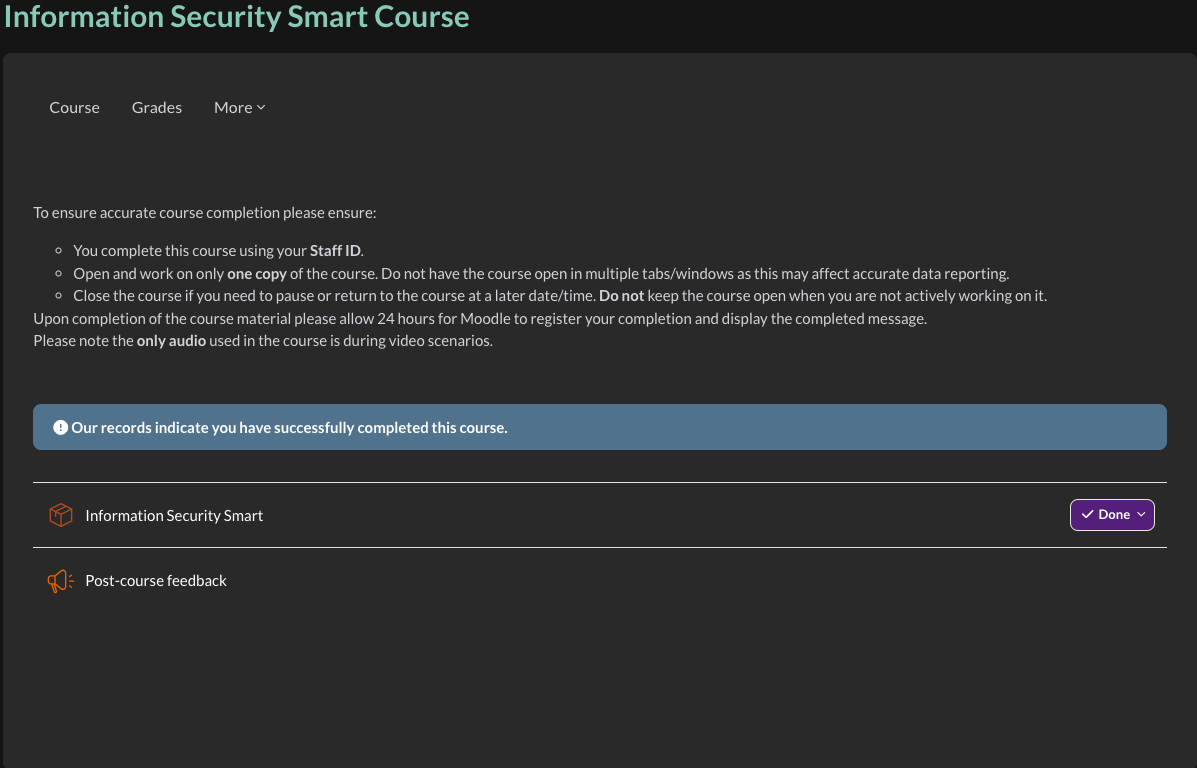
\includegraphics[width=1\textwidth]{images/information-security-smart-certificate.png}
    \caption{Information SMART certificate}
\end{figure}

\newpage

\subsection*{Appendix 3: Project plan}
\addcontentsline{toc}{subsection}{Appendix 3: Project plan}
\label{sec:Appendix 3}

\begin{longtable}{|p{5cm}|p{6cm}|p{4cm}|}
    \hline
    \textbf{Phase} & \textbf{Tasks} & \textbf{Duration} \\
    \hline
    \endfirsthead
    \hline
    \textbf{Phase} & \textbf{Tasks} & \textbf{Duration} \\
    \hline
    \endhead
    
    \hline
    \endfoot
    
    \hline
    \endlastfoot
    
    Research and Planning & 
    \begin{itemize}
        \item Conduct literature review.
        \item Refine research questions and objectives.
        \item Identify datasets (e.g., PhishTank, Kaggle).
    \end{itemize} & 
    End Jan – Early Feb (1–2 weeks) \\
    \hline
    
    Dataset Preparation & 
    \begin{itemize}
        \item Clean and preprocess data.
        \item Perform feature extraction (e.g., URLs, metadata).
        \item Split data into training, validation, and test sets.
    \end{itemize} & 
    Early Feb (1–2 weeks) \\
    \hline
    
    Model Development & 
    \begin{itemize}
        \item Develop baseline model (e.g., Random Forest, Logistic Regression).
        \item Experiment with advanced models (e.g., BERT).
        \item Train and validate models.
    \end{itemize} & 
    Mid-Feb – Early Mar (3 weeks) \\
    \hline
    
    Integration of XAI & 
    \begin{itemize}
        \item Implement SHAP and LIME for interpretability.
        \item Visualize explanations (e.g., feature importance, email components).
        \item Ensure explanation clarity and usability.
    \end{itemize} & 
    Early Mar – Mid-Mar (2 weeks) \\
    \hline
    
    Evaluation and Comparison & 
    \begin{itemize}
        \item Evaluate model performance (accuracy, F1-score).
        \item Assess interpretability using metrics (faithfulness, stability).
        \item Compare XAI-enhanced system to black-box models.
    \end{itemize} & 
    Mid-Mar – End Mar (2 weeks) \\
    \hline
    
    Report Writing & 
    \begin{itemize}
        \item Write methodology, results, and discussion sections.
        \item Proofread and finalize dissertation.
        \item Integrate appendices (e.g., Gantt chart, ethical approval).
    \end{itemize} & 
    April – Mid-May (5–6 weeks) \\
    \hline
    
    \end{longtable}
    


\end{document}
